% questions.tex —— 2007 年·普通高等学校招生考试·广东卷·理科 · 题目内容片段（无答案）
% 由 tools/generate_projects.py 依来源总账自 2007/2007_数学真题_广东理_试题.md 生成，勿手改（改源 MD 后重跑）


\gkpart{一、选择题}

\begin{question}
\gkti{1}已知函数 $f(x)=\dfrac{1}{\sqrt{1-x}}$ 的定义域为 $M$，$g(x)=\ln(1+x)$ 的定义域为 $N$，则 $M\cap N=$（　）

（A）$\{x\mid x>-1\}$

（B）$\{x\mid x<1\}$

（C）$\{x\mid -1<x<1\}$

（D）$\varnothing$

\end{question}
\begin{question}
\gkti{2}若复数 $(1+b\mathrm i)(2+\mathrm i)$ 是纯虚数（$\mathrm i$ 是虚数单位，$b$ 是实数），则 $b=$（　）

（A）$2$

（B）$\dfrac12$

（C）$-\dfrac12$

（D）$-2$

\end{question}
\begin{question}
\gkti{3}若函数 $f(x)=\sin^2x-\dfrac12$（$x\in\mathbf R$），则 $f(x)$ 是（　）

（A）最小正周期为 $\dfrac{\pi}{2}$ 的奇函数

（B）最小正周期为 $\pi$ 的奇函数

（C）最小正周期为 $2\pi$ 的偶函数

（D）最小正周期为 $\pi$ 的偶函数

\Needspace{0.4\textheight}
\end{question}
\begingroup
\renewenvironment{question}{\Needspace{0.5\textheight}}{}
\begin{question}
\gkti{4}客车从甲地以 $60\ \mathrm{km/h}$ 的速度匀速行驶 $1$ 小时到达乙地，在乙地停留了半小时，然后以 $80\ \mathrm{km/h}$ 的速度匀速行驶 $1$ 小时到达丙地。下列描述客车从甲地出发，经过乙地，最后到达丙地所经过的路程 $s$ 与时间 $t$ 之间关系的图象中，正确的是（　）
\nopagebreak[4]
\begin{center}% 2007 年广东卷理科第 4 题：四个 s-t 图象选项（A）—（D）。
%   客车：0—1 h 以 60 km/h 行驶（s: 0→60），1—1.5 h 停留（s=60），
%   1.5—2.5 h 以 80 km/h 行驶（s: 60→140）。
%   （A）第二段升到 160；（C）无停留段；（D）第二段斜率偏小、约 2.75 h 才到 140；
%   （B）三段折线与解析式一致。
% 来源 PDF：gaokaomath-src/普通高考/2007/2007广东理.pdf
% SHA-256：655db04340f14b909d7f248531436d45dd8cbd71e69aca976c3bd2d1e568ceed
% 原页：2007广东理.pdf 第 1 页（A3 三栏）第 1 栏，书页码 371，图在第 4 题题干下方。
% 重绘依据：按原页四个小图的折线顶点逐个比对；网格 0.25 h × 20 km，
%   横轴 0—3 h、纵轴 0—160 km，各图第二段斜率差异按原图保留。
\begin{tikzpicture}[x=0.95cm, y=0.024cm, semithick,
  every node/.style={inner sep=1.5pt}]

  % ---------------- 单个小图的公共网格 ----------------
  \newcommand{\stgrid}{%
    \foreach \gx in {0.25,0.5,...,3.0} {\draw[gray!45,very thin] (\gx,0) -- (\gx,160);}%
    \foreach \gy in {20,40,...,160} {\draw[gray!45,very thin] (0,\gy) -- (3.05,\gy);}%
    \draw[->,>=stealth] (0,0) -- (3.55,0) node[below right=1pt] {$t$ (h)};%
    \draw[->,>=stealth] (0,0) -- (0,178) node[left] {$s$ (km)};%
    \foreach \tx in {1,2,3} {\node[below] at (\tx,0) {$\tx$};}%
    \foreach \ty in {60,80,100,120,140,160} {\node[left] at (0,\ty) {$\ty$};}%
    \node[below left] at (0,0) {$O$};%
  }

  % ---------------- （A） ----------------
  \begin{scope}[shift={(0cm,0cm)}]
    \stgrid
    \draw[line width=1.1pt] (0,0) -- (1,60) -- (1.5,60) -- (2.5,160);
    \node at (1.7,-32) {（A）};
  \end{scope}

  % ---------------- （B） ----------------
  \begin{scope}[shift={(5.4cm,0cm)}]
    \stgrid
    \draw[line width=1.1pt] (0,0) -- (1,60) -- (1.5,60) -- (2.5,140);
    \node at (1.7,-32) {（B）};
  \end{scope}

  % ---------------- （C） ----------------
  \begin{scope}[shift={(0cm,-5.8cm)}]
    \stgrid
    \draw[line width=1.1pt] (0,0) -- (1,60) -- (2.5,140);
    \node at (1.7,-32) {（C）};
  \end{scope}

  % ---------------- （D） ----------------
  \begin{scope}[shift={(5.4cm,-5.8cm)}]
    \stgrid
    \draw[line width=1.1pt] (0,0) -- (1,60) -- (1.5,60) -- (2.75,140);
    \node at (1.7,-32) {（D）};
  \end{scope}
\end{tikzpicture}
\end{center}
\nopagebreak[4]
\end{question}
\endgroup
\begin{question}
\gkti{5}已知数列 $\{a_n\}$ 的前 $n$ 项和 $S_n=n^2-9n$，第 $k$ 项满足 $5<a_k<8$，则 $k=$（　）

（A）$9$

（B）$8$

（C）$7$

（D）$6$

\Needspace{0.4\textheight}
\end{question}
\begingroup
\renewenvironment{question}{\Needspace{0.35\textheight}}{}
\begin{question}
\gkti{6}图 1 是某县参加 $2007$ 年高考的学生身高条形统计图，从左到右的各条形表示的学生人数依次记为 $A_1$，$A_2$，$\cdots$，$A_{10}$（如 $A_2$ 表示身高（单位：$\mathrm{cm}$）在 $[150,155)$ 内的学生人数）。图 2 是统计图 1 中身高在一定范围内学生人数的一个算法流程图。现要统计身高在 $160\sim180\ \mathrm{cm}$（含 $160\ \mathrm{cm}$，不含 $180\ \mathrm{cm}$）的学生人数，那么在流程图中的判断框内应填写的条件是（　）
\nopagebreak[4]
\begin{center}% 2007 年广东卷理科第 6 题：图 1 身高条形统计图。
%   十组 [145,150)—[190,195)，人数依次 A1—A10 =
%   100、200、320、450、550、500、360、220、80、40（按原页柱高读取）。
%   原点处纵轴刻度由 0 折断到 50，图下 0 为人数原点，横轴标签为各柱左右分界。
% 来源 PDF：gaokaomath-src/普通高考/2007/2007广东理.pdf
% SHA-256：655db04340f14b909d7f248531436d45dd8cbd71e69aca976c3bd2d1e568ceed
% 原页：2007广东理.pdf 第 1 页（A3 三栏）第 2 栏，书页码 371。
% 重绘依据：横轴每格 5 cm、纵轴每格 50 人；0 与 50 之间按原图加折断线。
\begin{tikzpicture}[x=0.75cm, y=0.0085cm, semithick,
  every node/.style={inner sep=1.5pt, font=\small}]

  % 纵轴网格与刻度
  \foreach \gy in {50,100,...,600} {
    \draw[gray!45, very thin] (0,\gy) -- (11,\gy);
    \node[left] at (0,\gy) {\gy};
  }
  \draw[->,>=stealth] (0,0) -- (11.9,0) node[right] {身高/cm};
  \draw[->,>=stealth] (0,0) -- (0,660) node[above] {人数/人};

  % 原点折断线（0 与 50 之间）
  \draw (0,0) -- (0,20);
  \draw[white, line width=3pt] (-0.18,32) -- (0.18,32);
  \draw (-0.22,42) -- (0,32) -- (0.22,42);

  % 十根柱子：第 i 根覆盖 [145+5(i-1), 145+5i)
  \foreach \i/\h in {1/100,2/200,3/320,4/450,5/550,6/500,7/360,8/220,9/80,10/40} {
    \draw (\i,0) rectangle (\i+1,\h);
  }

  % 横轴标签：0 为原点，145—195 为各柱分界
  \node[below] at (0,0) {$0$};
  \foreach \i in {1,...,11} {
    \node[below] at (\i,0) {$\the\numexpr 140+5*\i\relax$};
  }

  \node at (5.5,-105) {图 1};
\end{tikzpicture}
\end{center}
\nopagebreak[4]
\nopagebreak[4]
\begin{center}% 2007 年广东卷理科第 6 题：图 2 算法流程图。
%   开始 → 输入 A1,A2,…,A10 → s=0,i=4 → 判断框（题目待填条件）→
%   是 → s=s+A_i → i=i+1 → 回到判断框上方；
%   否 → 输出 s → 结束。
% 来源 PDF：gaokaomath-src/普通高考/2007/2007广东理.pdf
% SHA-256：655db04340f14b909d7f248531436d45dd8cbd71e69aca976c3bd2d1e568ceed
% 原页：2007广东理.pdf 第 1 页（A3 三栏）第 2 栏，书页码 371。
% 重绘依据：按原页流程与分支方向重绘；判断框内留空，对应题目要求填写的条件。
\begin{tikzpicture}[scale=1.0, semithick,
  every node/.style={inner sep=2pt},
  box/.style={draw, rounded corners=2pt, minimum width=2.1cm,
    minimum height=0.55cm, align=center},
  para/.style={draw, trapezium, trapezium left angle=70,
    trapezium right angle=110, minimum width=2.9cm, minimum height=0.55cm,
    align=center},
  dec/.style={draw, diamond, aspect=2.6, minimum width=2.8cm,
    minimum height=1.05cm, align=center},
  arr/.style={->, >=stealth}]

  \node[box]  (start) at (0,8.6) {开始};
  \node[para] (in)    at (0,7.8) {输入 $A_1,A_2,\cdots,A_{10}$};
  \node[box]  (init)  at (0,6.9) {$s=0,\ i=4$};
  \node[dec]  (test)  at (0,5.5) {};
  \node[box]  (add)   at (4.6,4.9) {$s=s+A_i$};
  \node[box]  (inc)   at (4.6,6.1) {$i=i+1$};
  \node[para] (out)   at (0,3.9) {输出 $s$};
  \node[box]  (end)   at (0,3.0) {结束};

  \draw[arr] (start) -- (in);
  \draw[arr] (in) -- (init);
  \draw[arr] (init) -- (test);
  \draw[arr] (test.east) -- node[above] {是} (add.west);
  \draw[arr] (add.north) -- (inc.south);
  \draw[arr] (inc.west) -- (0,6.1) -- (0,6.32);
  \draw[arr] (test.south) -- node[left] {否} (out.north);
  \draw[arr] (out) -- (end);

  \node[below] at (2.6,2.55) {图 2};
\end{tikzpicture}
\end{center}
\nopagebreak[4]
（A）$i<6$

（B）$i<7$

（C）$i<8$

（D）$i<9$

\Needspace{0.4\textheight}
\end{question}
\endgroup
\begin{question}
\gkti{7}如图是某汽车维修公司的维修点环形分布图。公司在年初分配给 $A$，$B$，$C$，$D$ 四个维修点某种配件各 $50$ 件。在使用前发现需将 $A$，$B$，$C$，$D$ 四个维修点的这批配件分别调整为 $40$，$45$，$54$，$61$ 件，但调整只能在相邻维修点之间进行，那么要完成上述调整，最少的调动件次（$n$ 件配件从一个维修点调整到相邻维修点的调动件次为 $n$）为（　）
\nopagebreak[4]
\begin{center}% 2007 年广东卷理科第 7 题：维修点环形分布图。
%   A（左上）、D（右上）、C（右下）、B（左下）四点为环形相邻关系。
% 来源 PDF：gaokaomath-src/普通高考/2007/2007广东理.pdf
% SHA-256：655db04340f14b909d7f248531436d45dd8cbd71e69aca976c3bd2d1e568ceed
% 原页：2007广东理.pdf 第 1 页（A3 三栏）第 2 栏，书页码 371。
% 重绘依据：四点以椭圆节点表示，相邻点之间用弧线连接成环，环序 A—D—C—B—A。
\begin{tikzpicture}[scale=1.0, semithick,
  every node/.style={inner sep=1.5pt},
  pt/.style={draw, ellipse, minimum width=0.72cm, minimum height=0.44cm,
    align=center}]

  \node[pt] (A) at (-1.5,0.95) {$A$};
  \node[pt] (D) at (1.5,0.95)  {$D$};
  \node[pt] (B) at (-1.5,-0.95) {$B$};
  \node[pt] (C) at (1.5,-0.95) {$C$};

  \draw (A.east) .. controls (-0.6,1.75) and (0.6,1.75) .. (D.west);
  \draw (D.south) .. controls (2.15,0.3) and (2.15,-0.3) .. (C.north);
  \draw (C.west) .. controls (0.6,-1.75) and (-0.6,-1.75) .. (B.east);
  \draw (B.north) .. controls (-2.15,-0.3) and (-2.15,0.3) .. (A.south);
\end{tikzpicture}
\end{center}
\nopagebreak[4]
（A）$15$

（B）$16$

（C）$17$

（D）$18$

\end{question}
\begin{question}
\gkti{8}设 $S$ 是至少含有两个元素的集合。在 $S$ 上定义了一个二元运算“$*$”（即对任意的 $a$，$b\in S$，对于有序元素对 $(a,b)$，在 $S$ 中有唯一确定的元素 $a*b$ 与之对应）。若对任意的 $a$，$b\in S$，有 $a*(b*a)=b$，则对任意的 $a$，$b\in S$，下列等式中不恒成立的是（　）

（A）$(a*b)*a=a$

（B）$[a*(b*a)]*(a*b)=a$

（C）$b*(b*b)=b$

（D）$(a*b)*[b*(a*b)]=b$

\end{question}
\gkpart{二、填空题}

\begin{question}
\gkti{9}甲、乙两个袋中装有红、白两种颜色的小球，这些小球除颜色外完全相同。其中甲袋装有 $4$ 个红球，$2$ 个白球，乙袋装有 $1$ 个红球，$5$ 个白球。现分别从甲、乙两袋中各随机取出一个球，则取出的两球是红球的概率为\gkblank{}。（答案用分数表示）

\end{question}
\begin{question}
\gkti{10}若向量 $\boldsymbol a$，$\boldsymbol b$ 满足 $|\boldsymbol a|=|\boldsymbol b|=1$，$\boldsymbol a$，$\boldsymbol b$ 的夹角为 $120^\circ$，则 $\boldsymbol a\cdot\boldsymbol a+\boldsymbol a\cdot\boldsymbol b=$\gkblank{}。

\end{question}
\begin{question}
\gkti{11}在平面直角坐标系 $xOy$ 中，有一定点 $A(2,1)$。若线段 $OA$ 的垂直平分线过抛物线 $y^2=2px$（$p>0$）的焦点，则该抛物线的准线方程是\gkblank{}。

\Needspace{0.4\textheight}
\end{question}
\begin{question}
\gkti{12}如果一个凸多面体是 $n$ 棱锥，那么这个凸多面体的所有顶点所确定的直线共有\gkblank{}条。这些直线中共有 $f(n)$ 对异面直线，则 $f(4)=$\gkblank{}；$f(n)=$\gkblank{}。（答案用数字或 $n$ 的解析式表示）
\nopagebreak[4]
\begin{center}% 2007 年广东卷理科第 12 题：n 棱锥示意图（图中按五棱锥绘制）。
%   顶点 S 与底面五边形 A—B—C—D—E 相连；被遮挡的侧棱 S—E 与
%   底面后侧两条边画虚线。
% 来源 PDF：gaokaomath-src/普通高考/2007/2007广东理.pdf
% SHA-256：655db04340f14b909d7f248531436d45dd8cbd71e69aca976c3bd2d1e568ceed
% 原页：2007广东理.pdf 第 1 页（A3 三栏）第 3 栏，书页码 371。
% 重绘依据：按原页棱锥的顶点位置、虚实线与底面透视重绘。
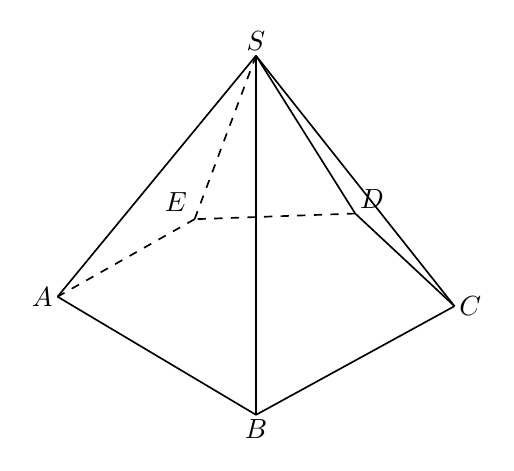
\begin{tikzpicture}[scale=1.2, semithick,
  every node/.style={inner sep=1.5pt}]

  \coordinate (S)  at (0,2.45);
  \coordinate (A)  at (-2.1,-0.10);
  \coordinate (B)  at (0,-1.35);
  \coordinate (C)  at (2.1,-0.20);
  \coordinate (D)  at (1.05,0.78);
  \coordinate (E)  at (-0.65,0.72);

  % 可见的侧棱
  \draw (S) -- (A);
  \draw (S) -- (B);
  \draw (S) -- (C);
  \draw (S) -- (D);
  % 被遮挡的侧棱
  \draw[dashed] (S) -- (E);

  % 可见的底边
  \draw (A) -- (B);
  \draw (B) -- (C);
  \draw (C) -- (D);
  % 被遮挡的底边
  \draw[dashed] (D) -- (E);
  \draw[dashed] (E) -- (A);

  \node[above] at (S) {$S$};
  \node[left]  at (A) {$A$};
  \node[below] at (B) {$B$};
  \node[right] at (C) {$C$};
  \node[above right] at (D) {$D$};
  \node[above left=1pt] at (E) {$E$};
\end{tikzpicture}
\end{center}
\nopagebreak[4]
\end{question}
\begin{question}
\gkti{13}在平面直角坐标系 $xOy$ 中，直线 $l$ 的参数方程为 $\begin{cases}x=t+3,\\ y=3-t,\end{cases}$（参数 $t\in\mathbf R$），圆 $C$ 的参数方程为 $\begin{cases}x=2\cos\theta,\\ y=2\sin\theta+2,\end{cases}$（参数 $\theta\in[0,2\pi)$），则圆 $C$ 的圆心坐标为\gkblank{}，圆心到直线 $l$ 的距离为\gkblank{}。

\end{question}
\begin{question}
\gkti{14}设函数 $f(x)=|2x-1|+x+3$，则 $f(-2)=$\gkblank{}；若 $f(x)\leqslant5$，则 $x$ 的取值范围是\gkblank{}。

\Needspace{0.4\textheight}
\end{question}
\begin{question}
\gkti{15}如图所示，圆 $O$ 的直径 $AB=6$，$C$ 为圆周上一点，$BC=3$。过点 $C$ 作圆的切线 $l$，过 $A$ 作 $l$ 的垂线 $AD$，$AD$ 分别与直线 $l$，圆交于点 $D$，$E$，则 $\angle DAC=$\gkblank{}，线段 $AE$ 的长为\gkblank{}。
\nopagebreak[4]
\begin{center}% 2007 年广东卷理科第 15 题：圆 O、切线 l、垂线 AD，AD 与圆交于 E。
%   直径 AB=6（半径 3），BC=3 给出圆心角 ∠BOC=60°，
%   C=(1.5,2.598)，过 C 的切线垂直于 OC，A 到切线的垂足 D=(-0.75,3.897)，
%   AD 与圆的另一个交点 E=(-1.5,2.598)。
% 来源 PDF：gaokaomath-src/普通高考/2007/2007广东理.pdf
% SHA-256：655db04340f14b909d7f248531436d45dd8cbd71e69aca976c3bd2d1e568ceed
% 原页：2007广东理.pdf 第 1 页（A3 三栏）第 3 栏，书页码 371。
% 重绘依据：按题设几何关系计算坐标后重绘；直角标记在 D 处，AB 直径水平。
\begin{tikzpicture}[scale=0.95, semithick,
  every node/.style={inner sep=1.5pt}]

  \coordinate (O) at (0,0);
  \coordinate (A) at (-3,0);
  \coordinate (B) at (3,0);
  \coordinate (C) at (1.5,2.598);
  \coordinate (D) at (-0.75,3.897);
  \coordinate (E) at (-1.5,2.598);

  \draw[thick] (O) circle (3);
  \fill (O) circle (1.2pt);
  % 直径 AB、弦 AC、A 到切线的垂线 AD（经过 E）
  \draw (A) -- (B);
  \draw (A) -- (C);
  \draw (A) -- (D);
  % 过 C 的切线 l（沿 D→C 方向并向右下延长）
  \draw (D) -- (C) -- (3.55,1.32);
  % 直角标记（AD ⊥ l）
  \coordinate (P1) at ($(D)!0.22cm!(C)$);
  \coordinate (P2) at ($(D)!0.22cm!(A)$);
  \draw (P1) -- ($(P1)+(P2)-(D)$) -- (P2);

  \node[left]  at (A) {$A$};
  \node[right] at (B) {$B$};
  \node[above right] at (C) {$C$};
  \node[above] at (D) {$D$};
  \node[below] at (O) {$O$};
  \node[left] at (E) {$E$};
  \node[right] at (3.55,1.32) {$l$};
\end{tikzpicture}
\end{center}
\nopagebreak[4]
\end{question}
\gkpart{三、解答题}

\begin{question}
\gkti{16}已知 $\triangle ABC$ 顶点的直角坐标分别为 $A(3,4)$，$B(0,0)$，$C(c,0)$。

（1）若 $c=5$，求 $\sin\angle A$ 的值；

（2）若 $\angle A$ 是钝角，求 $c$ 的取值范围。

\end{question}
\begin{question}
\gkti{17}下表提供了某厂节能降耗技术改造后生产甲产品过程中记录的产量 $x$（吨）与相应的生产能耗 $y$（吨标准煤）的几组对照数据。

\begin{center}
\begin{tabular}{lllll}
\toprule
$x$ & $3$ & $4$ & $5$ & $6$ \\
\midrule
$y$ & $2.5$ & $3$ & $4$ & $4.5$ \\
\bottomrule
\end{tabular}
\end{center}

（1）请画出上表数据的散点图；

（2）请根据上表提供的数据，用最小二乘法求出 $y$ 关于 $x$ 的线性回归方程 $\hat y=\hat b x+\hat a$；

（3）已知该厂技改前 $100$ 吨甲产品的生产能耗为 $90$ 吨标准煤。试根据（2）求出的线性回归方程，预测生产 $100$ 吨甲产品的生产能耗比技改前降低多少吨标准煤？

（参考数值：$3\times2.5+4\times3+5\times4+6\times4.5=66.5$）

\end{question}
\begin{question}
\gkti{18}在平面直角坐标系 $xOy$ 中，已知圆心在第二象限，半径为 $2\sqrt2$ 的圆 $C$ 与直线 $y=x$ 相切于坐标原点 $O$。椭圆 $\dfrac{x^2}{a^2}+\dfrac{y^2}{9}=1$ 与圆 $C$ 的一个交点到椭圆两焦点的距离之和为 $10$。

（1）求圆 $C$ 的方程；

（2）试探究 $C$ 上是否存在异于原点的点 $Q$，使 $Q$ 到椭圆右焦点 $F$ 的距离等于线段 $OF$ 的长。若存在，请求出点 $Q$ 的坐标；若不存在，请说明理由。

\Needspace{0.4\textheight}
\end{question}
\begin{question}
\gkti{19}如图所示，等腰 $\triangle ABC$ 的底边 $AB=6\sqrt6$，高 $CD=3$，点 $E$ 是线段 $BD$ 上异于点 $B$，$D$ 的动点，点 $F$ 在 $BC$ 边上，且 $EF\perp AB$，现沿 $EF$ 将 $\triangle BEF$ 折起到 $\triangle PEF$ 的位置，使 $PE\perp AC$，记 $BE=x$，$V(x)$ 表示四棱锥 $P-ACFE$ 的体积。

（1）求 $V(x)$ 的表达式；

（2）当 $x$ 为何值时，$V(x)$ 取得最大值？

（3）当 $V(x)$ 取得最大值时，求异面直线 $AC$ 与 $PF$ 所成角的余弦值。
\nopagebreak[4]
\begin{center}% 2007 年广东卷理科第 19 题：等腰三角形沿 EF 折起后的四棱锥 P-ACFE。
%   底面三角形 ABC 中 D 为 AB 中点，CD=3，AB=6√6；
%   E 在 DB 上，F 在 BC 上，EF∥CD；△BEF 沿 EF 折起，B 的对应点为 P，
%   P 在 E 正上方；虚线为被遮挡的底边 AE 与底面内的高 CD。
% 来源 PDF：gaokaomath-src/普通高考/2007/2007广东理.pdf
% SHA-256：655db04340f14b909d7f248531436d45dd8cbd71e69aca976c3bd2d1e568ceed
% 原页：2007广东理.pdf 第 2 页（A3 三栏）第 2 栏，书页码 372。
% 重绘依据：按原页折起后的投影关系重绘，保持 A、C、B、D、E、F、P 的相对位置。
\begin{tikzpicture}[scale=0.95, semithick,
  every node/.style={inner sep=1.5pt}]

  \coordinate (A) at (-4.0,0);
  \coordinate (B) at (4.0,0);
  \coordinate (C) at (0,-2.6);
  \coordinate (D) at (0,0);
  \coordinate (E) at (1.8,0);
  \coordinate (F) at (1.8,-1.43);
  \coordinate (P) at (1.8,3.0);

  % 原三角形 ABC 的底边与边
  \draw[dashed] (A) -- (E);
  \draw (E) -- (B);
  \draw (A) -- (C);
  \draw (C) -- (B);

  % 底面内的高 CD（被遮挡）
  \draw[dashed] (C) -- (D);

  % 折痕与四棱锥的侧棱
  \draw (E) -- (F);
  \draw (P) -- (A);
  \draw (P) -- (C);
  \draw (P) -- (F);
  \draw (P) -- (E);

  % 标注
  \node[left]  at (A) {$A$};
  \node[right] at (B) {$B$};
  \node[below] at (C) {$C$};
  \node[above=1pt] at (D) {$D$};
  \node[right] at (E) {$E$};
  \node[below right] at (F) {$F$};
  \node[above] at (P) {$P$};
\end{tikzpicture}
\end{center}
\nopagebreak[4]
\end{question}
\begin{question}
\gkti{20}已知 $a$ 是实数，函数 $f(x)=2ax^2+2x-3-a$。如果函数 $y=f(x)$ 在区间 $[-1,1]$ 上有零点，求 $a$ 的取值范围。

\end{question}
\begin{question}
\gkti{21}已知函数 $f(x)=x^2+x-1$，$\alpha$，$\beta$ 是方程 $f(x)=0$ 的两个根（$\alpha>\beta$），$f'(x)$ 是 $f(x)$ 的导数，设 $a_1=1$，$a_{n+1}=a_n-\dfrac{f(a_n)}{f'(a_n)}$（$n=1,2,\cdots$）。

（1）求 $\alpha$，$\beta$ 的值；

（2）证明：对任意的正整数 $n$，都有 $a_n>\alpha$；

（3）记 $b_n=\ln\dfrac{a_n-\beta}{a_n-\alpha}$（$n=1,2,\cdots$），求数列 $\{b_n\}$ 的前 $n$ 项和 $S_n$。

\end{question}